%-----------------------------------------------------------------------------
%	PACKAGES AND THEMES
%-----------------------------------------------------------------------------
\documentclass[aspectratio=169,xcolor=dvipsnames]{beamer}
\usetheme{SimplePlus}

\usepackage[utf8]{inputenc}
\usepackage{hyperref}
\usepackage{graphicx}
\usepackage{booktabs}
\usepackage[serbian]{babel}
\usepackage{pgfplots}


%-----------------------------------------------------------------------------
%	TITLE PAGE
%-----------------------------------------------------------------------------

\title[short title]{Capture The Flag (CTF)}
\subtitle{CTF kao uvod u računarsku bezbednost}

\author[andrija] {Andrija Urošević, prof: dr. Sana Stojanović Đurđević}

\institute[matf]
{
    Računarstvo i društvo\\
    Univerzitet u Beogradu\\
    Matematički fakultet
}
\date{April, 2022.}


%-----------------------------------------------------------------------------
%	PRESENTATION SLIDES
%-----------------------------------------------------------------------------

\begin{document}

\begin{frame}
    \titlepage
\end{frame}

\begin{frame}{Pregled}
    \tableofcontents
\end{frame}

%-----------------------------------------------------------------------------
\section{CTF takmičenja}
%-----------------------------------------------------------------------------

\begin{frame}{CTF takmičenje}

    \begin{block}{Capture The Flag (CTF)}
        \emph{Capture The Flag} (CTF) je takmičenje u oblasti računarske 
        bezbednosti. Cilj takmičenja je pronaći \emph{flag}-ove u nekom 
        okruženju.
    \end{block}

    \begin{block}{Flag}
        \emph{Flag} je tipično neki string karaktera, čiju specifikaciju daju
        organizatori takmičenja. \emph{Flag} obično ima neki prefiks.
    \end{block}

    \begin{exampleblock}{Primer Flag-a}
        Prefiks: \texttt{FLAG} \\
        \emph{Flag}: \texttt{FLAG\{K73BSSxY3nFc1oAs9WwG\}}
    \end{exampleblock}


\end{frame}

%-----------------------------------------------------------------------------

\begin{frame}{Vrste CTF takmičenja}

    \begin{block}{Jeopardy}
        U \emph{Jeopardy} CTF-u, takmičari dobiju unapred zadate zadatke, 
        koji su statični.
    \end{block}

    \begin{block}{Attack-Defence}
        \emph{Attack-Defence} stil podrazumeva borbu između timova. Svaki 
        tim ima sopstvenu mrežu koja ima ranjive servise. Cilj je ``zakrpiti'' 
        ranjive servise, i u isto vreme eksploatisati druge timove. 
    \end{block}

    \begin{block}{Mixed}
        \emph{Mixed} CTF može biti različitog formata, ali kao što ime sugeriše 
        predstavlja mešavinu prethodna dva stila.
    \end{block}
    
\end{frame}

%-----------------------------------------------------------------------------

\begin{frame}{Popularna CTF takmičenja}

    \begin{exampleblock}{CTF takmičenja}
        DEFCON CTF, UCSB iCTF, Mozilla CTF, Facebook CTF, Google CTF, PHD CTF, 
        RuCTFe, Hack.lu CTF, SECUINSIDE CTF, rwth CTF, CSAW CTF, PICO CTF,...,
        DESCON CTF \cite{ctftime} \cite{ctfdescon}
    \end{exampleblock}

    \begin{figure}
        \begin{center}
            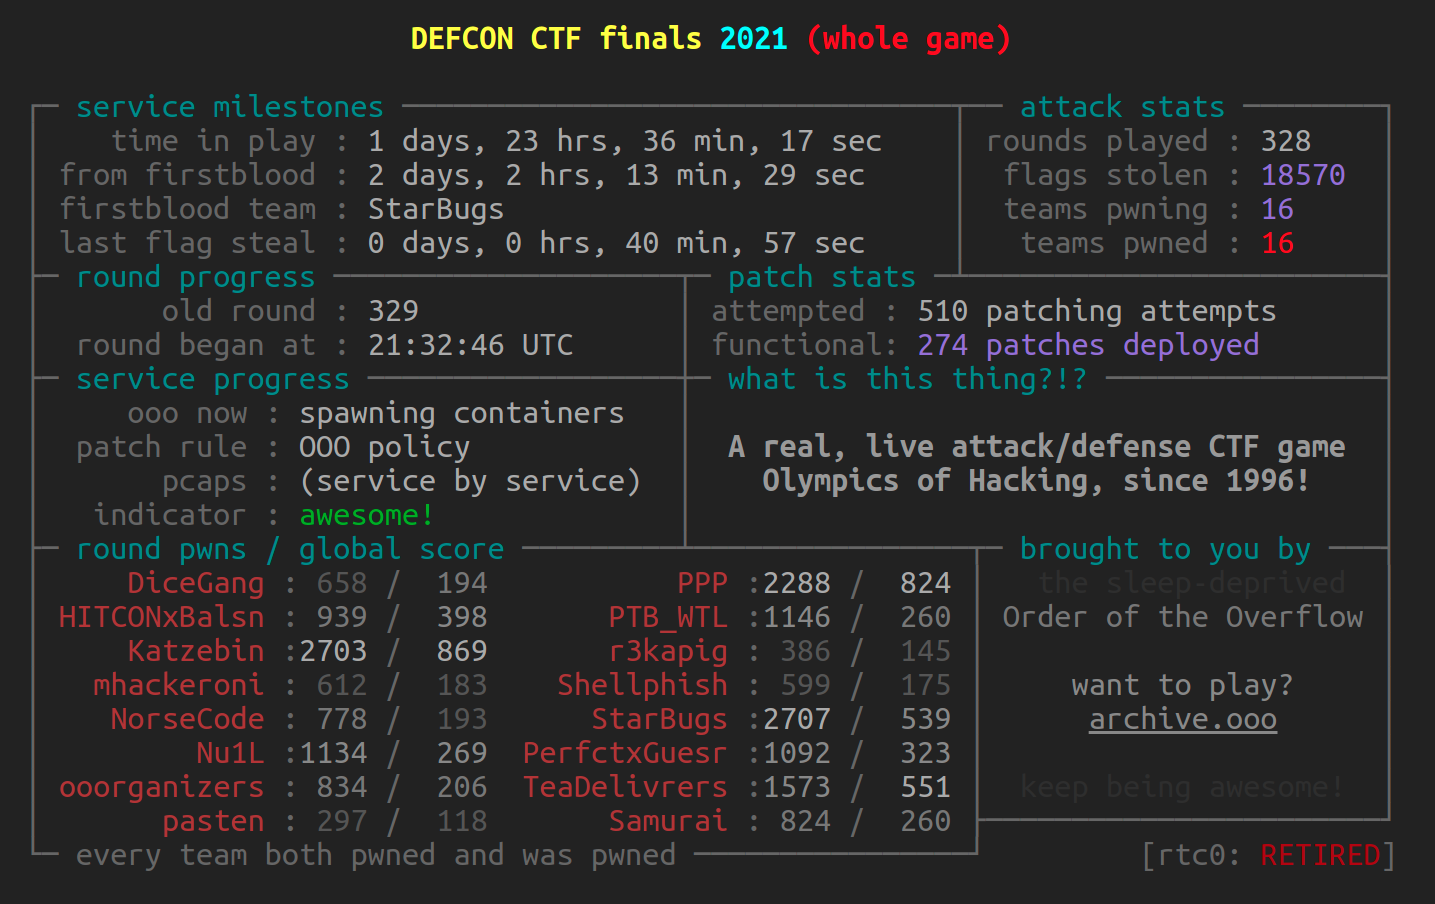
\includegraphics[width=0.4\textwidth]{Slike/ctf_comp.png}
        \end{center}
        \caption{DEFCON CTF finale 2021}
    \end{figure}

\end{frame}

%-----------------------------------------------------------------------------
\section{Znanja i veštine koje se stiču kroz CTF}
%-----------------------------------------------------------------------------

\begin{frame}{CSEC2017 oblasti znanja}

    \begin{block}{CyberSecurity Curricula 2017}
        \cite{ctfcsec17} definiše osam oblasti znanja u računarskoj bezbednosti:
        \begin{enumerate}
            \item Bezbednost podataka
            \item Bezbednost softvera 
            \item Bezbednost komponenti
            \item Bezbednost konekcije
            \item Bezbednost sistema
            \item Bezbednost ljudi
            \item Organizaciona bezbednost
            \item Društvena bezbednost
        \end{enumerate}
    \end{block}

\end{frame}

%-----------------------------------------------------------------------------

\begin{frame}{Distribucija oblasti znanja u CTF zadacima}
    \begin{figure}
        \begin{center}
            \begin{tikzpicture}[scale=0.6]
                \begin{axis}[
                        y=1cm, 
                        xbar, 
                        title={Distribucija oblasti znanja u CTF-u}, 
                        symbolic y coords={
                            Društvo, 
                            Organizacija, 
                            Ljudi, 
                            Sistemi, 
                            Konekcije, 
                            Komponente, 
                            Softver, 
                            Podaci
                        },
                        legend pos = south east, 
                        nodes near coords, 
                        xmax=50
                    ]
                    \addplot+ coordinates {
                        (2.96,Društvo) 
                        (9.86,Organizacija) 
                        (8.23,Ljudi) 
                        (12.72,Sistemi) 
                        (19.66,Konekcije) 
                        (8.94,Komponente) 
                        (10.02,Softver) 
                        (27.61,Podaci)
                    }; 
                    \addlegendentry{Jeopardy}
                    \addplot+ coordinates {
                        (2.17,Društvo) 
                        (11.38,Organizacija) 
                        (9.18,Ljudi) 
                        (10.96,Sistemi) 
                        (32.68,Konekcije) 
                        (2.08,Komponente) 
                        (14.72,Softver) 
                        (16.83,Podaci)
                    }; 
                    \addlegendentry{Attack-Defence}
                \end{axis}
            \end{tikzpicture}
        \end{center}
        \caption{
            Distribucija oblasti znanja u $15 879$ \emph{jeopardy} i 
            $86$ \emph{attack-defense} \emph{writeup}-ova.\cite{ctfskills}
        }\label{fig:ctf_ka}
    \end{figure}
\end{frame}

%-----------------------------------------------------------------------------
\section{Problemi u CTF modelu}
%-----------------------------------------------------------------------------

\begin{frame}{Problemi u CTF modelu}
    \cite{ctfchung} pronalaze sledeće probleme u CTF modelu:
    \begin{enumerate}
        \item Težina igre
        \item Relacija između dizajna zadataka i njegove uspešnosti pri
            rešavanju
        \item Dokaz o kvalitetu
        \item Poeni i njihov obrnuti efekat na takmičare i organizatore
        \item Infrastruktura zadataka
        \item Dvosmisleni zadaci
    \end{enumerate}
\end{frame}

%-----------------------------------------------------------------------------
\section{CTF na univerzitetskim kursevima}
%-----------------------------------------------------------------------------

\begin{frame}{CTF na univerzitetskim kursevima}
    \begin{table}[!h]
        \centering
        \begin{tabular}{|c|c|c|}
            \hline
            \textbf{Osobina} & \textbf{CTF} & \textbf{CCTF} \\
            \hline
            \hline
            Pripremanje & nekoliko meseci & nekoliko nedelja \\
            Trajanje & 1-2 dana & 2 časa \\
            Uloge timova & crveni ili plavi & crveni i plavi \\
            Uparivanje timova & svi na sve & parovi \\
            Učestalost & jednom godišnje & 2-3 puta po semestru \\
            Analiza & retko & uvek \\
            Težina & stručni & početni do srednji \\
            \hline
        \end{tabular}
        \caption{Upoređivanje CTF-a i CCTF-a.\cite{ctfclass}}\label{tab:cctf}
    \end{table}
\end{frame}

%-----------------------------------------------------------------------------

\begin{frame}{Poboljšanje edukacija kroz CTF}

    \cite{ctfleune} u svom radu pokazuju sledeće hipoteze:
    \begin{enumerate}
        \item Samopouzdanje studenata će se povećati učestvovanjem u CTF-u.
        \item Studenti će uživati u CTF-u.
        \item Studenti će steći praktične veštine učestvovanjem u CTF-u.
        \item Učestvovanje u CTF potkrepljuje teorijske koncepte.
    \end{enumerate}

\end{frame}

%-----------------------------------------------------------------------------

\begin{frame}{Prednosti i mane CTF-a na kursevima}

    \cite{ctfuni}:
    \begin{itemize}
        \item Performanse studenata
        \item Korisno navođenje
        \item Deljenje CTF \emph{flag}-ova
        \item CTF igre sa studentske strane
    \end{itemize}

\end{frame}

%-----------------------------------------------------------------------------
\section{Zaključak}
%-----------------------------------------------------------------------------

\begin{frame}{Zaključak}
    \begin{alertblock}{Gamifikacija kroz CTF}
        Gamifikacija u obliku CTF-a se pokazuje kao veoma dobar alat za 
        učenje o računarskoj bezbednosti, uz savladive probleme koje donosi.
    \end{alertblock}
\end{frame}

%-----------------------------------------------------------------------------

\begin{frame}{Reference}
    \footnotesize{
        \begin{thebibliography}{99}
            \bibitem[CTFTime.org]{ctftime} CTFTime
                \newblock All about CTF (Capture The Flag)
                \newblock \emph{ctftime.org}

            \bibitem[DESCON.me]{ctfdescon} DESCON CTF
                \newblock DESCON IoT Hackathon
                \newblock \emph{descon.me}

            \bibitem[OverTheWire.org]{ctfwire} Over The Wire
                \newblock We're hackers, and we are good-looking. We are 1\%.
                \newblock \emph{overthewire.org}

        \end{thebibliography}
    }
\end{frame}

%-----------------------------------------------------------------------------

\begin{frame}{Reference}
    \footnotesize{
        \begin{thebibliography}{99}
            \bibitem[CSEC2017]{ctfcsec17} CyberSecurity Curricula 2017
                \newblock Curriculum Guidelines for Post-Secondary Degree
                Programs in Cybersecurity
                \newblock \emph{Joint Task Force}

            \bibitem[Švabenski i dr. 2021.]{ctfskills} Švábenský, Valdemar i 
                Celeda, Pavel i Vykopal, Jan i Brisakova, Silvia
                \newblock Cybersecurity Knowledge and Skills Taught in 
                Capture the Flag Challenges
                \newblock \emph{Elsevier Computers \& Security}, 2021.

            \bibitem[Čang i Koen, 2021.]{ctfchung} Kevin Chung i Julian Cohen
                \newblock Learning Obsticles in the Capture The Flag Model
                \newblock \emph{USENIX Sumit on Gaming, Games, and 
                Gamification in Security Education}, 2014.

        \end{thebibliography}
    }
\end{frame}

%-----------------------------------------------------------------------------

\begin{frame}{Reference}
    \footnotesize{
        \begin{thebibliography}{99}
            \bibitem[Mirković i Piterson, 2014.]{ctfclass} Jelena Mirković i 
                Peter A. H. Peterson.
                \newblock Class Capture-the-Flag Exercises
                \newblock \emph{USENIX Summit on Gaming, Games, and 
                Gamification in Security Education}, 2014.

            \bibitem[Leune i Petrilli, 2017.]{ctfleune} Kees Leune i 
                Salvatore J. Petrilli
                \newblock Using Capture-the-Flag to Enhance the Effectivness
                of Cybersecurity Education
                \newblock \emph{Proceeding of the 18th Annual Conference
                on Information Technology Education}, str. 47-52, 2017.
            \bibitem[Vikopa i dr, 2020.]{ctfuni} Jan Vykopal, Valdemar 
                Švábenský i Ee-Chien Chang
                \newblock Benefits and Pitfalls of Using Capture the Flag
                Games in University Courses
                \newblock 2020.

        \end{thebibliography}
    }
\end{frame}

%-----------------------------------------------------------------------------

\begin{frame}
    \Huge{\centerline{\textbf{Pitanja?}}}
\end{frame}

%-----------------------------------------------------------------------------

\end{document}
